%-
%*----------- SLIDE -------------------------------------------------------------
\begin{frame}[t]{Resultados}
    \transdissolve[duration=0.5]
    % \begin{table}
    %   \begin{tabular}{ c c c }
    %     Parameters           &	 3 wheels  &  4 wheels \\
    %     d (m)                &   0.0       &  89       \\
    %     r (m)                &   0.0       &  325      \\ 
    %     l                    &             &  5        \\
    %     $K_v (V /(rad/s))$ &   0.0       &  259      \\
    %     R (Ω)                &   4.3       &  111      \\
    %     M (kg)               &   1.944     &  2.34     \\
    %     J (kg · m2 )         &   0.0169    &  0.0228   \\
    %     $B_v (N/(m/s))$    &   0.5082    &  0.4978   \\
    %     $B_{vn} (N/(m/s))$ &   0.4870    &  0.6763   \\
    %     $B_ω (N · m/(rad/s))$ &0.0130    &  0.0141   \\
    %     $C_v (N)$          &   1.9068    &  1.8738   \\
    %     $C_{vn} (N)$       &   2.0423    &  2.2198   \\
    %     $C_ω (N · m)$      &   0.0971    &  0.1385 
    %   \end{tabular}
    % \end{table}
    \begin{figure}[ht!]
      \centering
  
      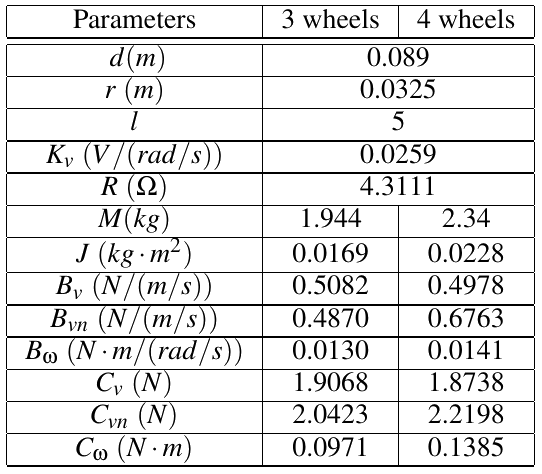
\includegraphics[width=0.9\textheight]{table.png}
      \label{fig:result_table}
  
    \end{figure}
  
    %*----------- notes
    \note[item]{Notes can help you to remember important information. Turn on the notes option.}
  \end{frame}


%*----------- SLIDE -------------------------------------------------------------
\begin{frame}[t]{Resultados}
  \transdissolve[duration=0.5]

  \begin{figure}[ht!]
    \centering
    \begin{subfigure}[b]{0.4\textwidth}
      \centering
      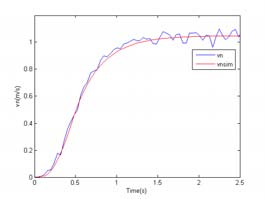
\includegraphics[width=\textwidth]{result_graph_3w_vn.png}
      % \roundpic[xshift=0cm,yshift=0cm]{4.5cm}{4.5cm}{Three_wheeled_robot.png}
      \caption{Velocidade no eixo vn.}
      \label{fig:result_3w_vn}
    \end{subfigure}
    ~
    \begin{subfigure}[b]{0.4\textwidth}
      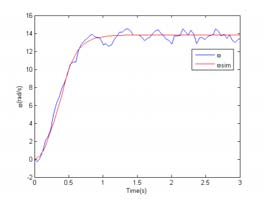
\includegraphics[width=\textwidth]{result_graph_3w_w.png}
      % \roundpic[xshift=0cm,yshift=0cm]{4.5cm}{4.5cm}{four_wheeled_robot.png}
      \caption{Velocidade em rotação.}
      \label{fig:result_3w_w}
    \end{subfigure}    
  \caption{Validação do modelo (3 rodas).}
  \end{figure}
  
  %*----------- notes
  \note[item]{Notes can help you to remember important information. Turn on the notes option.}
\end{frame}

%*----------- SLIDE -------------------------------------------------------------
\begin{frame}[t]{Resultados}
  \transdissolve[duration=0.5]

  \begin{figure}[ht!]
    \centering
    \begin{subfigure}[b]{0.4\textwidth}
      \centering
      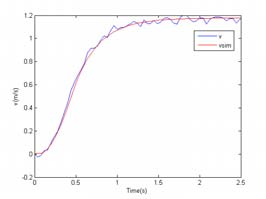
\includegraphics[width=\textwidth]{result_graph_4w_v.png}
      % \roundpic[xshift=0cm,yshift=0cm]{4.5cm}{4.5cm}{Three_wheeled_robot.png}
      \caption{Velocidade no eixo v.}
      \label{fig:result_4w_v}
    \end{subfigure}
    ~
    \begin{subfigure}[b]{0.4\textwidth}
      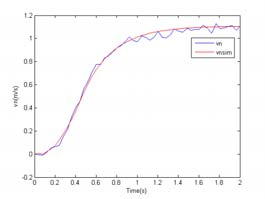
\includegraphics[width=\textwidth]{result_graph_4w_vn.png}
      % \roundpic[xshift=0cm,yshift=0cm]{4.5cm}{4.5cm}{four_wheeled_robot.png}
      \caption{Velocidade no eixo vn.}
      \label{fig:result_4w_vn}
    \end{subfigure}    
  \caption{Validação do modelo (4 rodas).}
  \end{figure}
  
  %*----------- notes
  \note[item]{Notes can help you to remember important information. Turn on the notes option.}
\end{frame}